Much of machine learning is concerned with the analysis of given data. By contrast, the fields of optimal experiment design (OED) and active learning are concerned with the creation of new data by experimentation or query. In many contexts, careful design of the experiment leads to more efficient learning. The gain in efficiency can be dramatic -- rendering previously infeasible experimental programs feasible. (citation needed)

Idealised active learning can be represented as follows
\begin{center}
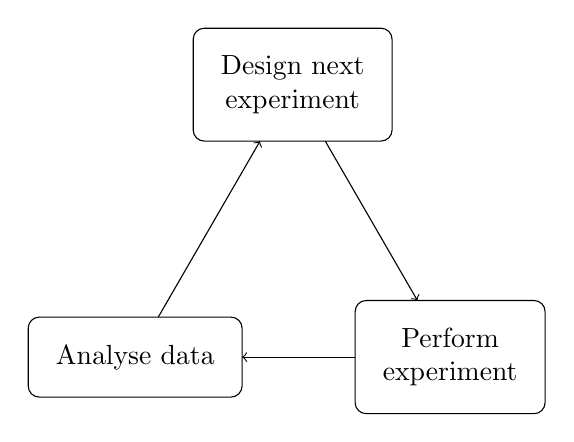
\begin{tikzpicture}
	[every node/.style={inner sep=10,outer sep=0,rounded corners}]
	\node (design) [draw, align=center] at (0, 0) {Design next \\ experiment};
	\node (perform) [draw, align=center] at (2, -3.46) {Perform \\ experiment};
	\node [draw] (analyse) at (-2, -3.46) {Analyse data};
	\draw [->] (design) -- (perform);
	\draw [->] (perform) -- (analyse);
	\draw [->] (analyse) -- (design);
\end{tikzpicture}
\end{center}
It is only within the context of a proposed data analysis that the optimality or suboptimality of an experiment design can be assessed.

\section{Foundations}
\subsection{Problem specification}
We assume the data analysis model for the experiment takes the form given by the graphical model
\begin{center}
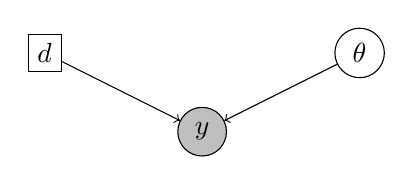
\begin{tikzpicture}
	\tikzstyle{every node}=[draw,shape=circle]
	\node[draw,fill=lightgray] (y) at (0, 0) {$y$};
	\node (t) at (2, 1) {$\theta$};
	\node[draw,shape=rectangle] (d) at (-2, 1) {$d$};
	\draw [->] (d) -- (y);
	\draw [->] (t) -- (y);
\end{tikzpicture}
\end{center}
in which $d$ represents the (non-random) design of the experiment, $\theta$ represents a latent variable and $y$ represents the observed outcome of the experiment. The joint density is
\begin{equation}
	p(y, \theta | d) = p(\theta)p(y|\theta,d)
\end{equation}
We can generalize to the sequential design setting by 
standard Bayesian updating, namely at experiment iteration $t$, we replace $p(\theta)$ with 
$p(\theta | d_{1:t-1}, y_{1:t-1})$, where $d_{1:t-1}$ and  $y_{1:t-1}$ are the designs and outcomes at previous steps of the experiment.
The likelihood $p(y_t | \theta, d_t)$ is assumed unchanged. That is, experimentation does not change the behaviour of the underlying system from time to time, conditional upon $\theta$.


\subsection{One-step design}
Suppose we assign a real-valued utility $U(y, \theta, d)$ to the event of observing $y$ under design $d$ when the true latent variable was $\theta$. We can average over $y$ to obtain
\begin{equation}
	U(\theta, d) = \int p(y | \theta, d)\ U(y, \theta, d)\ dy
\end{equation}
We can deal with $\theta$ in various ways
\begin{itemize}
	\item The Bayesian approach \cite{chaloner1995} places a prior $p(\theta)$ on $\theta$ and takes $U(d) = \int p(\theta)\ U(\theta, d)\ d\theta$
	\item The minimax approach \cite{fedorov1972} takes $U(d) = \inf_\theta U(\theta, d)$
	\item The local approach \cite{pronzato2010} begins with an estimate $\hat{\theta}$ and sets $U(d) = U(\hat{\theta}, d)$
\end{itemize}
The optimal design would then be
\begin{equation}
	d^* = \argmax_{d \in \mathcal{D}} \ U(d)
\end{equation}
where $\mathcal{D}$ is the space of admissible designs. Here, we primarily focus on the Bayesian approach. This is not an arbitrary decision, it can be motivated from decision theoretic considerations \cite{lindley1972}. See \cite{chaloner1995}, \cite{ryan2015} for further discussion of Bayesian experimental design.

Alternatively, we could take the (matrix-valued) `utility'
\begin{equation}
	U(y, \theta, d) = \left( \frac{\partial}{\partial \theta} \log p(y | \theta, d) \right)^2
\end{equation}
which leads to the the Fisher Information Matrix, used in many experiment design criteria \cite{pronzato2010}, defined as
\begin{equation}
	\mathcal{I}(\theta, d) = \int \left( \frac{\partial}{\partial \theta} \log p(y | \theta, d) \right)^2 p(y | \theta, d)\ dy
\end{equation}
We can obtain a scalar utility from $\mathcal{I}(\theta, d)$ by choosing from the `alphabetical' criteria \cite{box1982} which are defined as
\begin{itemize}
	\item D-optimality $U(d, \theta) = \text{det } \mathcal{I}(\theta, d)$
	\item A-optimality $U(d, \theta) = \text{tr } \mathcal{I}(\theta, d)$
	\item E-optimality $U(d, \theta) = \max_i \lambda_i$ where $\lambda_i$ are the eigenvalues of $\mathcal{I}(\theta, d)$
\end{itemize}

Work dating back to \cite{lindley1956} instead uses an information-theoretic utility\footnote{It can also be shown \cite{chaloner1995} that this utility leads to a (modified form) of D-optimality for linear models.}
\begin{equation}
	U(y, \theta, d) = \log \frac{p(\theta | y, d)}{p(\theta)} = \log \frac{p(y | \theta, d)}{p(y|d)}
\end{equation}
and Lindley established that this is the only form that satisfies certain intuitive properties of an informative experiment. For this reason, we will focus on this utility. See \cite{ryan2015} for a fuller discussion of utility functions used in experiment design.

With the information-theoretic utility and Bayesian averaging, we arrive at the following form for $U(d)$, called the \textbf{expected information gain (EIG)}
\begin{equation}
	U(d) = \eig(d) = \iint p(y, \theta | d) \log\frac{p(\theta | y, d)}{p(\theta)} \ dy\ d\theta
\end{equation}
The EIG can be interpreted in a number of ways
\begin{enumerate}
\item As the expectation of information gain. If we define
\begin{equation}
	\text{IG}(y, d) = \text{KL}(\ p(\theta | y, d)\ ||\ p(\theta)\ ) 
\end{equation}
then $\eig(d) = \expect_{y\sim p(y|d)}[\text{IG}(y, d)] $.
\item From APE. Define the \textbf{average posterior entropy} (APE) as 
\begin{align}
	\ape(d) &= \iint p(y, \theta | d) \log p(\theta | y, d) \ dy \ d\theta \\
	&= -\int p(y|d) \entropy{p(\theta | y, d)} dy
\end{align}
where $H$ is the differential entropy.
Then
\begin{equation}
	\eig(d) = \entropy{p(\theta)} - \ape(d)
\end{equation}
and the prior entropy is a constant w.r.t. $d$. Thus EIG maximisation corresponds to APE
minimisation.
\item Mutual information. Recall the mutual information is defined as
\begin{equation}
	\text{MI}(x, y) = \kl{p(x, y)}{p(x)p(y)}
\end{equation}
then we have
\begin{align}
	\text{MI}(y, \theta | d) &= \kl{p(y, \theta | d)}{p(y|d)p(\theta)} \\
	&= \iint p(y, \theta | d) \log \frac{p(y, \theta | d)}{p(\theta)p(y|d)} dy \, d\theta \\
	&= \eig(d)
\end{align}
\item Epistemic uncertainty.
The total entropy or uncertainty in response $y$ is
\begin{equation}
	\entropy{p(y|d)}
\end{equation}
the aleatoric uncertainty under parameter $\theta$ is
\begin{equation}
	\entropy{p(y|\theta, d)}
\end{equation}
Under prior $p(\theta)$, the expected aleatoric uncertainty is
\begin{equation}
	\expect_{\theta \sim p(\theta)}\left[ \entropy{p(y|\theta, d)} \right]
\end{equation}
The epistemic uncertainty, under $p(\theta)$, is
\begin{align}
	&\entropy{p(y|d)} - \expect_{\theta \sim p(\theta)}\left[ \entropy{p(y|\theta, d)} \right] \\
	=&-\int p(y|d)\log p(y|d)dy + \iint p(y, \theta | d)\log p(y|\theta, d) dy \, d\theta\\
	=& \eig(d)
\end{align}

\end{enumerate}
We shall see that the connection to mutual information in particular is handy for estimating EIG, because modern techniques for estimating MI have been developed in the recent past.


\subsection{Multi-step design}
Designing a sequence of multiple experiments, with a view to maximise expected utility can be viewed as a Partially Observable Markov Decision Process (POMDP), and falls within the scope of reinforcement learning \cite{pang2018}. The problem is also referred to as backward induction or stochastic dynamic programming. The formal reframing of OED as a POMDP is laid out below.

\subsubsection{Setup}
Suppose we have a determinic, finite time horizon $t=1, ..., T$. We specify as Partially Observable Markov Decision Process (POMDP) as follows.
\begin{itemize}
\item States $s_t = (\theta, h_t)$, where $h_t = d_{1:t}, y_{1:t}$ the history of designs $d$ and outcomes $y$ up to the current time. Here $y_t \sim p(y | \theta, d)$ is the outcome of performing the experiment using design $d_t$. The practical state $s'_t$ consists of the sufficient statistics for $\theta$ obtained from $h_t$. These can be used to compute the belief states $b_t$, encoding the full posterior for $\theta$ given that history $h_t$.
\item Actions $a_t = d_{t+1}$. Transitions correspond to running the experiment and producing the outcome $Y_{t+1}$.
\item Observations $o_t = h_t$. Thus the only unobserved part of the state $(\theta, h_t)$ is the latent $\theta$.
\item Rewards $r_t = r(t, \theta, h_t)$. We take $r$ to be a non-random function. Note that in many OED settings, we take $r_t = 0$ for $t<T$. Intuitively, this means we only care about our final understanding of or action upon the system, not the path taken to it. This is the choice made by \cite{gonzalez2016} among others.
\end{itemize}
Under this set-up, the \textit{optimal experiment design policy} is a $\pi$ from histories $h_t$ to actions $a_t$ which maximises the total reward
\begin{equation}
	R_T = \expect \left[ \sum_{t=1}^T \gamma^t r_t \mid \pi \right]
\end{equation}
where $\gamma \in [0,1]$ is the discount factor. In a finite horizon setting, we typically set this to 1. When there are only terminal rewards and $\gamma=1$, this reduces to
\begin{equation}
	\label{eq:terminalreward}
	R_T = \expect[r_T \mid \pi]
\end{equation}


\subsubsection{Connection to EIG}
\paragraph{Horizon 1}
Suppose $T=1$. Choose the following reward function
\begin{equation}
r(1, \theta, h) = \log \frac{p(\theta | y, d)}{p(\theta)} = \log \frac{p(y | \theta, d)}{p(y|d)}
\end{equation}
The $Q$-function of action $d_1$ is the expected reward
\begin{equation}
	Q(s_0, d_1) = E_{y \sim p(y|\theta, d)}[r(t, \theta, d_1, y)]
\end{equation}
Since we have no observation of $\theta$, the belief $Q$-function of the belief state $p(\theta)$ and action $d_1$ is
\begin{equation}
	Q(p(\theta), d_1) = E_{\theta \sim p(\theta)}\{E_{y \sim p(y|\theta, d)}[r(t, \theta, d_1, y)]\}
\end{equation}
which reduces to the familiar expression
\begin{equation}
	Q(p(\theta), d_1) = \iint p(y, \theta | d) \log \frac{p(\theta | y, d)}{p(\theta)} \, d\theta \, dy
\end{equation}

\paragraph{Horizon $T$}
This formalism provides a convenient way to avoid the greedy approach to sequential design that is compatible with the information-theoretic objective of \cite{lindley1956}.

Suppose the belief at time $t$ is $b_t(\theta)$. This can be computed from the sufficient stats $s'_t$. We take the reward to be $0$ at $t<T$ and
\begin{equation}
	r(T, \theta, h_T) = r(T, \theta, b_T(\theta)) = \log \frac{b_T(\theta) }{p(\theta)}
\end{equation}
we have updated $b$ according to Bayes Theorem so
\begin{equation}
	b_T(\theta) = p(\theta | y_{1:T}, d_{1:T})
\end{equation}
This reward structure represents the total information gained about $\theta$ from all experiments.

In fact, we can rewrite this reward to take non-zero values at earlier times, setting
\begin{equation}
	\label{eq:rlmutli}
	r(t, \theta, h_t) = r(t, \theta, b_t(\theta)) = \log\frac{b_t(\theta)}{b_{t-1}(\theta)}
\end{equation}
and this is equivalent to the previous formulation. To see this, consider the belief $Q$-function
\begin{align}
	Q(b_t(\theta), d_{t+1}) =& \int b_t(\theta)  \int p(y_{t+1} | \theta, d_{t+1}) \log\frac{b_{t+1}(\theta)}{b_t(\theta)} \\ &+ \int p(y_{t+2} | \theta, d_{t+1}, y_{t+1}) \log \frac{b_{t+2}(\theta)}{b_{t+1}(\theta)} + \hdots \, dy_{t+2} \, dy_{t+1} \, d\theta \\
	=& \int b_t(\theta) \int p(y_{t+1:t+2}|\theta, d_{t+1}) \log \frac{b_{t+2}(\theta)}{b_t(\theta)} + \hdots \, dy_{t+1:t+2} \, d\theta \\
	=& \hdots \\
	=& \int b_t(\theta) \int p(y_{t+1:T}|\theta,d_{t+1}) \log \frac{b_T(\theta)}{b_t(\theta)} \, dy_{t+1:T} \, d\theta
\end{align}
where $p(y_{t+1:T}|\theta, d_{t+1})$ assumes an optimal strategy after step $t+1$, under reward \eqref{eq:rlmutli}. We can now see by induction that the optimal strategy and $Q$-functions are the same for either choice of reward structure.

\subsubsection{The greedy approach}
In reinforcement learning, greediness refers to maximising the one-step-ahead reward, namely
\begin{equation}
	a_t = \argmax_{a_t \in \mathcal{A}} \left(\expect[r_{t+1} | a_t] \right)
\end{equation}
which, with the reward of \eqref{eq:rlmutli}, corresponds to one-step EIG maximisation at each step. We primarily focus on this form of multi-step optimisation because it removes all aspects of future planning beyond a single step from an already difficult problem.

\subsubsection{Non-greedy approaches}
Some have considered non-greedy strategies \cite{gonzalez2016} \cite{pang2018}. See \cite[sec 6.1]{ryan2015} for a summary of `backwards induction' approaches.


\subsubsection{Optional stopping}

We finally mention another possible complication. Rather than a fixed and finite time horizon $T$, we may we allowed to continue experimentation indefinitely, choosing when to stop. One natural choice to stopping criterion is to terminate when the posterior entropy reaches a threshold value.


\subsection{Theoretical considerations}
The proposed experimentation strategy in which we design future experiments on the basis of previous observations may, at first sight, cause some consternation to the theoretical statistician. The first question we seek to answer is `in what sense is the posterior obtained from multi-step OED the same as that obtained by a pre-ordained experimentation strategy?' The second line of questioning concerns the asymptotics of multi-step OED. `Is multi-step OED statistically consistent and does it provide a faster convergence rate than other methods?'

To the first question, the answer is simply that the posterior is the same as if the experimentation strategy had been pre-ordained. Indeed, let us regard the designs as random variables and consider a 2-step experiment with the following graphical model
\begin{center}
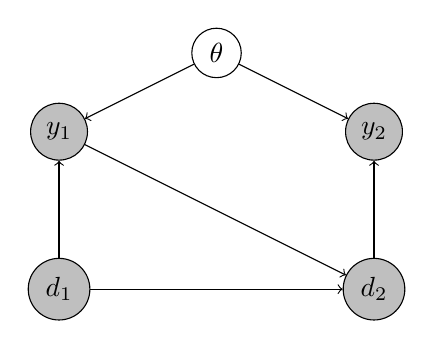
\begin{tikzpicture}
	\tikzstyle{every node}=[draw,shape=circle]
	\node (t) at (0, -1) {$\theta$};
	\node[draw,fill=lightgray] (y1) at (-2, -2) {$y_1$};
	\node[draw,fill=lightgray] (y2) at (2, -2) {$y_2$};
	\node[draw,fill=lightgray] (d1) at (-2, -4) {$d_1$};
	\node[draw,fill=lightgray] (d2) at (2, -4) {$d_2$};
	\draw [->] (d1) -- (y1);
	\draw [->] (t) -- (y1);
	\draw [->] (d2) -- (y2);
	\draw [->] (t) -- (y2);
	\draw [->] (d1) -- (d2);
	\draw [->] (y1) -- (d2);
\end{tikzpicture}
\end{center}
and the following conditional density for $\theta$
\begin{align}
	p(\theta | y_1, d_1, y_2, d_2) =& \frac{p(\theta, y_1, d_1, y_2, d_2)}{p(y_1, d_1, y_2, d_2)} \\
	=& \frac{p(\theta)p(d_1)p(y_1|\theta, d_1)p(d_2|y_1,d_1)p(y_2|\theta,d_2)}{\int p(\theta)p(d_1)p(y_1|\theta, d_1)p(d_2|y_1,d_1)p(y_2|\theta,d_2) d\theta} \\
	=& \frac{p(d_1)p(d_2|y_1,d_1)\ p(\theta)p(y_1|\theta, d_1)p(y_2|\theta,d_2)}{p(d_1)p(d_2|y_1,d_1)\ \int p(\theta)p(y_1|\theta, d_1)p(y_2|\theta,d_2) d\theta} \\
	=& \frac{p(\theta)p(y_1|\theta, d_1)p(y_2|\theta,d_2)}{\int p(\theta)p(y_1|\theta, d_1)p(y_2|\theta,d_2) d\theta}
\end{align}
showing that the dependence between $d_2$ and $d_1, y_1$ need not bother us. A related question from \cite{berry1985} was whether the map that takes the observed data to the posterior is a measurable function. This was addressed in \cite[pp. 18-20]{berry1985} in the restricted setting of the multi-armed bandit.

A powerful answer to the second question was given by \cite{paninski2005} and is a form of Bernstein--von Mises Theorem for EIG maximisation OED. Under relatively mild conditions, for any neighbourhood $\mathcal{U}$ of the true parameter value $\theta_0$ we have
\begin{equation}
	p(\mathcal{U} | y_{1:T}, d_{1:T}) \to 1 \text{ as } T \to \infty \text{ in probability}
\end{equation}
Under further conditions, we can show that the posteriors $p(\theta | y_{1:T}, d_{1:T})$ are asymptotically Normal with covariance matrix $\Sigma_\text{info}$. The same result holds for i.i.d. sampling of designs, giving rise to $\Sigma_\text{iid}$. We have that $\text{det}\ \Sigma_\text{info} \le \text{det}\ \Sigma_\text{iid}$. This led \cite{paninski2005} to say ``Thus, information maximization is in a rigorous sense asymptotically more efficient than the i.i.d. sampling strategy.'' Related results were obtained by \cite{pronzato2010} and \cite{hu1998}.

\section{Estimation of EIG}
The estimation of EIG, and quantities mathematically equivalent to it, has received attention from a diverse group of researchers.

\subsection{Challenges in EIG estimation}
Recall
\begin{align}
	\label{eig:post}
	\eig(d) =
	\iint  p(y, \theta | d) \log \frac{p(\theta | y, d)}{p(\theta)} \, dy\,  d\theta
	=\iint  p(y, \theta | d) \log \frac{p(y | \theta, d)}{p(y|d)} \, dy\,  d\theta.
\end{align}
The computation of this integral is challenging since neither $p(\theta|y,d)$ nor $p(y|d)$ nor the outer integral can, in general, be found in closed form.

A further complication arises when the likelihood $p(y|\theta,d)$ cannot be computed pointwise. For example, this is the case in the presence of nuisance variables, also known as random effects. 
These are additional latent variables, $\psi$, that we do not consider variables of interest and so we do not want to waste resources reducing our uncertainty for them. 
Such models arise frequently in scientific applications, for instance accounting for individual variation between participants in a survey. With random effects $\psi$ we have
\begin{equation}
	p(y|\theta, d) = \int p(y|\theta, \psi, d) p(\psi | \theta) d\psi
\end{equation}
which is typically intractable.

We survey existing approaches to EIG estimation.

\subsection{Nested Monte Carlo}
The estimator of \cite{vincent2017} and \cite{myung2013}, among others, is a nested Monte Carlo (NMC) estimator
\begin{equation}
	\eig(d) \approx \frac{1}{N}\sum_{n=1}^N \left[ \log p(y_n | \theta_n, d) - \log \left(\frac{1}{M} \sum_{m=1}^M p(y_n | \theta_m, d) \right) \right]
\end{equation}
where
\begin{align}
	y_n, \theta_n \simiid & \ p(y, \theta | d) \\
	\theta_m \simiid & \ p(\theta)
\end{align}
are all independent.

The drawbacks of such an estimator were noted in \cite{nmc}. Most notably, while simple Monte Carlo estimators converge with a mean squared error rate $\mathcal{O}(N^{-1})$ in the total number of samples, NMC estimators converge at a much slower $\mathcal{O}(N^{-2/3})$ rate and are biased, though consistent \cite{nmc}.

A saving grace of the MC approach is a speed-up due to \cite{vincent2017} in the case that $\mathcal{Y}$, the sample space of $y$, is finite. Then
\begin{equation}
	\eig(d) \approx \sum_y \left[ \frac{1}{N}\sum_{n=1}^N p(y | \theta_n, d) \log p(y | \theta_n, d) -  \left(\frac{1}{N} \sum_{n=1}^N p(y | \theta_n, d) \right) \log \left( \frac{1}{N} \sum_{n=1}^N p(y | \theta_n, d) \right) \right]
\end{equation}
where
\begin{equation}
	\theta_n \simiid \ p(\theta).
\end{equation}
Since this is a continuous function of vanilla Monte Carlo estimators, it converges at a rate $\mathcal{O}(N^{-1})$.

We finally mention that, whilst not present in the literature, NMC can be readily extended to the case of random effects
\begin{equation}
	\eig(d) \approx \frac{1}{N}\sum_{n=1}^N \left[ \log \left(\frac{1}{M'} \sum_{m'=1}^{M'} p(y_n | \theta_n, \psi_{nm'}, d) \right) - \log \left(\frac{1}{M} \sum_{m=1}^M p(y_n | \theta_m, \psi_m, d) \right) \right]
\end{equation}
where
\begin{align}
	y_n, \theta_n \simiid & \ p(y, \theta | d) \\
	\psi_{nm'} | \theta_n \sim & \ p(\psi | \theta_n) \\
	\theta_m, \psi_m \simiid & \ p(\theta, \psi)
\end{align}
and we note that we can replace $\psi_{nm'}$ with $\psi_m$ when $\theta$ and $\psi$ are independent under the prior $p(\theta, \psi)$. Again, when $\mathcal{Y}$ is finite a speed-up is possible, although we can no longer avoid nesting Monte Carlo estimators.

\subsection{Inference based approaches}
A number of authors \cite{long2013, ryan2015} use some form of Laplace approximation to $p(\theta|y,d)$ to estimate expected information gain. In \cite{ouyang2016}, probabilistic programming is used to completely solve the inference problem (in finite spaces) en route to estimating EIG.

\subsection{Mutual information estimation}
As mentioned previously, EIG estimation is mathematically equivalent to mutual information estimation, a topic that has received recent attention in part due to the connection with Generative Adversarial Networks (GANs) \cite{infogan} and disentanglement \cite{tianqichen}. In the following section, we drop $d$ from our graphical model, and consider a joint density $p(y, \theta) = p(\theta)p(y|\theta)$.

Since $p(\theta|y)$ is typically an intractable, we might use an approximation $q(\theta|y)$. An idea used by \cite{ba} and \cite{infogan} is to bound the mutual information in terms of an amortised posterior $q(\theta|y)$ as
\begin{align}
	\text{MI}(y, \theta) =& \int p(\theta) \int p(y|\theta) \log \frac{p(\theta | y)}{p(\theta)} \, dy \, d\theta \\
	\ge & \int p(\theta) \int p(y|\theta) \log \frac{q(\theta | y)}{p(\theta)} \, dy \, d\theta.
\end{align}
For a fuller derivation and discussion of this and related bounds, see Chapter~\ref{chap:voed} on variational optimal experiment design.

A more recent idea is to use the Donsker-Varadhan Representation of the KL divergence to estimate mutual information \cite{mine}. We have
\begin{equation}
	\label{eq:dv}
	\text{MI}(y, \theta) = \kl{p(y, \theta)}{p(y)p(\theta)} = \sup_T \left\{ \expect_{p(y,\theta)} [T(y, \theta)] - \log\left(\expect_{p(\theta)p(y)}[e^{T(y,\theta)}] \right)  \right\}
\end{equation}
where the supremum is taken over measurable $T$. Note that the optimising $T$ is given by
\begin{equation}
	T^*(y, \theta) = \log\frac{p(y,\theta)}{p(y)p(\theta)} + C \text{ where }C\text{ is any constant}
\end{equation}
The importance of \eqref{eq:dv} is that we no longer need access to any densities to estimate the mutual information.

Practical implementations arising from both these objective functions follow from choosing a suitable parametric family for $T$ (or, in the former case, for $q(\theta|y)$). One then optimises the bound w.r.t. the parameters of the family using finite sample approximations to the expectations. We note that such an idea is intimately connected with the GAN \cite{fgan}.

\section{Optimisation of EIG}
So far, little attention has been paid to the design $d$. We suppose now that $d \in \mathcal{D}$ and we seek
\begin{equation}
	d^* = \argmax_{d\in\mathcal{D}} \quad \eig(d)
\end{equation}
the optimal design. As outlined in the previous section, we can have only approximate estimates of $\eig(d)$. This puts us squarely in the domain of Bayesian optimisation \cite{shahriari2016}. When $\mathcal{D}$ is finite, we would term it a multi-armed bandit problem.

Bayesian optimisation in its simplest form requires
\begin{enumerate}
	\item A model of the unknown function
	\item An acquisition rule to decide which design(s) should be queried at the next iteration
\end{enumerate}
It is a fascinating fact that we are now back in the setting of OED. The variable of interest is the location of $d^*$, the maximiser of the unknown function. Other features of the function can be regarded as random effects. See \cite{pes} for further discussion on the connection between Bayesian optimisation and OED, in particular, the connection of EIG to Bayesian optimisation.

A popular approach to Bayesian optimisation is to choose a Gaussian process (GP) model of the unknown function, and an upper confidence bound (UCB) acquisition rule \cite{srinivas2009}.

One aspect that sets $\eig$ maximisation apart from conventional Bayesian optimisation is the ability for us to obtain more accurate estimates of the unknown function $\eig$ by varying the amount of computational resources assigned to estimation. This was explored by \cite{vincent2017} in a finite $\mathcal{D}$ setting. The number of NMC samples was increased for the most promising designs. \cite{mcleod2017} tackled a more general problem of variable cost objectives, taking a GP based approach.

\section{Applications}
TODO: Major revisions needed

\subsubsection{Machine learning and statistics}
There is long-standing interest in `classical' statistical models and their design \cite{youssefreview}. Consider a basic linear models with Gaussian noise. Optimal design here can be expressed in terms of the eigenspectrum of $XX^T$ (see \cite{chaloner1984}). For nonlinear models, see the section on Physics. What about GLMs? Likely can solve the problem analytically again. These are great baselines. People in the linear models case are often concerned with proving the equivalence of different kinds of optimality \cite{youssefreview}.

In machine learning, experiment design is closely related to two common techniques in, for example, image classification: data augmentation and active learning.

In data augmentation images are rotated, translated, etc to create more training data. We could theoretically optimise the augmentation but this seems wasteful since copying the labels to new images is very easy.

A much more interesting area is \textit{active learning}. In this context, there are a large number of unlabeled images. Labeling is expensive. We select which images to label either up front, or (more typical in active learning) in a sequential manner. The key difference here is that we have a finite pool of unlabeled instances. We may be more interested in reducing uncertainty in the labels of these unlabeled images than in our posterior entropy.

The connection between active learning and Bayesian optimal design was explored in \cite{golovin2010}. In this paper, they start from a place where the outcome of a test is deterministic (think of the 12 men on an island problem). In the noiseless setting, the sequential design can be encoded as a decision tree and the problem is called the Optimal Decision Tree problem. This problem is known to be NP-hard. The OED criterion is introduced later to account for noisy observations and the fact that true parameters need not be known exactly even after all tests have been run.

A particular active learning example can be found in \cite{nowak2009}. We have $\mathcal{H}$ a hypothesis space (read parameter space) and $\mathcal{X}$ a query space (read design space). The goal is to determine the true $h^* \in \mathcal{H}$. Each query outputs a label in $\{-1, 1\}$ corrupted with Bernoulli noise (independent between queries). The algorithm broadly works by targeting $x \in \mathcal{X}$ where the expected posterior label in near $0$ (random guess). The convergence rate of $\prob(\hat{h}_i \ne h^*) \to 0$ is studied (shown exponential). The importance of having access to unlabeled data is exploited by \cite{dasgupta2006}.

\subsubsection{Psychology}
For an overview of optimal experiment design in probabilistic programming, \cite{ouyang2016} from Noah's group is a good place to start. Experiment design is necessary to distinguish competing theories. We should select models with the highest \textit{expected information gain}, written formally as 
\begin{equation}
U(d) = \expect_{(Y, \Theta) \sim p(y, \theta | d)}\left\{\log \frac{p(\Theta | Y, d)}{p(\Theta)}\right\}
\end{equation}
This equation has been studied by mathematical statisticians since the 50's \cite{lindley1956}. We can naively evaluate $U(d)$ in a PPL via \textit{nested inference}.

A canonical experiment discussed in this paper is the 5-4 experiment for category learning \cite{medin1978}. The experiment aimed to distinguish two competing models of category learning: the \textit{exemplar model} (learn categories by comparing new items to all previous items) and the \textit{prototype model} (learn categories by remembering a prototypical example). There are two models, so $\Theta = \{m_1, m_2\}$. During the experiment, participants are presented with a sequence of objects. In the training phase, they are also told the correct label after guessing. In testing they have no feedback. The objects varied in four dimensions: colour, shape, size and count; we can consider the space of objects to be $\{0,1\}^4$. Each object has a label $A$ or $B$. The true labeling mechanism was limited by Medin and Schaffer to be linearly separable. There are 9 inputs in the final testing set and Medin and Schaffer restricted there to be 5 $A$s and 4 $B$s. The objects $0000$ and $1111$ have to be present. Under these restrictions there are 933 possible experiments up to permutation. So $\mathcal{D}$ is a finite set of size 933. $\mathcal{Y}$ is the `test' responses, ie. the subjects responses when they are not given feedback. Thus $\mathcal{Y} = \{A, B\}^9$. The kind of participant numbers seen were 10-30.

In \cite{vincent2017}, the canonical experiment is as follows. We want to model how humans discount future rewards relative to present ones (via utility indifference pricing framework). A single experiment takes the following form: `Would you prefer £$A_1$ at time $t_1$ or £$A_2$ at time $t_2$'? The parameter of interest is the discount factor. Formally, $\mathcal{D} = [0, \infty)^2$, $\mathcal{Y} = \{1, 2\}$ and $\Theta = [0, \infty)$. These three spaces fit together as follows. We first chose $\mathcal{D}$ the space of possible designs. We subsequently chose $\mathcal{Y}$ the space of possible outcomes. We posited a probabilistic model for $Y$ in terms of parameters $\theta$. Focus on non-nested estimation for finite $\mathcal{Y}$ and sequential design. Sequential design means different participants will be asked different questions based on their previous answers.

\subsubsection{Bioinformatics}

In \cite{vanlier2012}, the authors consider experiment design from the perspective that, with little data, many different parameter settings adequately describe the data. Canonical model. Biochemical network modeled as an ODE.
\begin{align*}
&\dot{x} = f(x, u, p) \\
&\dot{y} = g(x, q) + \xi \\
&x(0) = x_0
\end{align*}
$u$ is the input, $x, y$ are time varying (uncontrolled) with $x$ latent and $y$ observed, $p, q, x_0$ are parameters $\theta$ required to simulate the model and do not depend on $t$, $\xi$ represents measurement noise. We treat $\xi$ as iid Gaussian. The paradigm chosen here is expected variance reduction, as opposed to information gain. (Possibly wrong if people still do that.) The variance is in the posterior predictive density.

\subsubsection{Physics}
In \cite{berg2003}, we begin by discussing `classical' experiment design procedures which assume linear dependence between model and outcome $y = G_{m_0}d$. One can solve this linear equation by least squares, $\hat{d} = G^T(GG^T)^{-1}y$. Define $L = G^T(GG^T)^{-1}$, possibly adding regularization as necessary. Basically, you want to maximize the max eigenvalue of $G$, which is essentially a gradient. The larger gradient, the more informative the experiment. In a linear setting, the gradient does not depend on the true parameter value.

Now consider linear noise but a nonlinear function between parameters and outcomes. For example, the authors took
\begin{equation}
R_p = \left(\frac{1}{2}[1 + \tan^{-1} i] - 4c^2 \sin^2 i\right) \frac{\Delta \alpha}{\alpha}
\end{equation}
where $\alpha = (\alpha 1 + \alpha2)/2$, $\Delta \alpha = (\alpha 2 - \alpha 1)$. The parameter we want to optimize is $\alpha2$.

This is a relatively simple and comprehensible case.